\documentclass{article}
\usepackage[utf8]{inputenc}
\usepackage{mathrsfs}
\usepackage{tikz}
\usepackage{amssymb}
\usepackage{amsthm}
\usepackage{graphicx} % Required for inserting images
\usepackage{amsmath}
\usepackage{MnSymbol}
\usepackage{geometry}
\usepackage{physics}
\usepackage{enumerate}
\allowdisplaybreaks
\newcommand\numeq[1]%
  {\stackrel{\scriptscriptstyle(\mkern-1.5mu#1\mkern-1.5mu)}{=}}
\newcommand\numleq[1]
  {\stackrel{\scriptscriptstyle(\mkern-1.5mu#1\mkern-1.5mu)}{\leq}}
\newcommand\numgeq[1]
  {\stackrel{\scriptscriptstyle(\mkern-1.5mu#1\mkern-1.5mu)}{\geq}}

\newtheorem{definition}{Definition}[section]
\newtheorem{theorem}{Theorem}[section]
\newtheorem{remark}{Remark}[section]
\newtheorem{example}{Example}[section]



\title{Math 133 Homework 1}
\author{Thomas Slavonia}
\date{\today}

\begin{document}
\maketitle
\section*{1.}
\begin{proof}
Let $0 < r < 1$ and we look that the integral 
\[
 \int_0^r \frac{1}{1 + x^2} \mathrm{d}x. 
\]
Since $x^2 < 1$ always for $x \in [0, r]$ using power series expansion we have that 
\[
 \int_0^r \frac{1}{1 + x^2}\mathrm{d}x = \int_0^r \sum\limits_{n = 0}^{\infty} (-1)^n (x^2)^n \mathrm{d}x. 
\]
We can swap the integral and the sum if the series is uniformly convergent, and to find whether or not the series is uniformly convergent, we can use the Weierstrass M-test. So, 
\[
 \sum\limits_{n = 0}^{\infty} \left|x^{2n} \right| 
\]
will converge as $x < 1$, and then the ratio test shows convergence clearly. Thus, the series passes the Weierstrass M-test and is uniformly convergent. 
Hence, 
\[
 \int_0^r \sum\limits_{n = 0}^{\infty} (-1)^n x^{2n} \mathrm{d}x = \sum\limits_{n = 0}^{\infty} \int_0^r (-1)^n x^{2n} \mathrm{d}x = \sum\limits_{n = 0}^{\infty} (-1)^n \frac{r^{2n + 1}}{2n + 1}. 
\]
Consider the statement of Abels Theorem: if $\sup \sum\limits_{n = 0}^{\infty}a_nr^n$ is absolutely convergent and $\sum\limits_{n = 0}^{\infty}a_n$ is convergent, then 
\[
 \lim\limits_{r \to 1^-} \sum\limits_{n = 0}^{\infty}a_nr^n = \sum\limits_{n = 0}^{\infty} a_n \text{ exists}. 
\]
Proof of Abel's:\\
Define $S_N = \sum\limits_{j = 0}^{N}a_j$ as the partial sum. Then, 
\begin{align*}
  \sum\limits_{k = 0}^na_kr^k &= \sum\limits_{k = 0}^n (S_k - S_{k - 1})r^k \\
  &= \sum\limits_{k = 0}^nS_kr^k - \sum\limits_{k = 0}^nS_{k - 1}r^k \\
  &= \sum\limits_{k = 0}^{n - 1}S_kr^k - \sum\limits_{k = 0 }^{n - 1}S_kr^{k + 1} + S_nr^n\\
  &= (1 - r)\sum\limits_{k = 0}^{n - 1}S_kr^k + S_nr^n. 
\end{align*}
as $n \to \infty$, 
\[
 \lim\limits_{n \to \infty} \left((1 - r)\sum\limits_{k = 0}^{n - 1}S_kr^k + S_nr^n \right) = \sum\limits_{n = 0}^{\infty}a_kr^k
\]
converges and $\lim\limits_{n \to \infty}S_nr^n = 0$ as $r < 1$ and since $S_n$ is bounded we must have the convergence. Thus, for $|r| < 1$ the partial sums must converge, so 
\[
 \sum\limits_{k = 0}^{\infty}a_kr^k = (1 - r)\sum\limits_{k = 0}^{\infty}S_kr^k. 
\]
Since $S_k$ converges, $\forall \epsilon > 0$ $\exists N \in \mathbb{N}$ such that 
\[
 \left|(1 - r) \sum\limits_{k = N}^{\infty} S_kr^k \right| \leq \epsilon (1 - r) \sum\limits_{k = N}^{\infty}r^n = \epsilon (1 - r) \frac{1}{1 - r} = \epsilon 
\]
so we have controlled the latter part of the sum. 
Note that 
\[
 (1 - r)\sum\limits_{k = 0}^{N - 1}S_kr^k \to 0 \text{ as } r \to 1^- 
\]
and thus 
\[
 \lim\limits_{r \to 1^-}\sum\limits_{k = 0}^{\infty}a_kr^k = \sum\limits_{k = 0}^{\infty}a_k = \lim\limits_{r \to 1^-}(1 - r)\sum\limits_{k = 0}^{\infty}S_kr^k < 2 \epsilon.  
\]
So, Abel's theorem is true, and 
\[
 \sum\limits_{n =0 }^{\infty} (-1)^n \frac{r^{2n + 1}}{2n + 1}  
\]
converges by the alternating series test and meets all of the qualifications for Abel's theorem. Thus, $\lim\limits_{r \to 1^-}$ exists and 
\[
 \lim\limits_{r \to 1^-} \sum\limits_{n = 0}^{\infty}(-1)^n\frac{r^{2n + 1}}{2n+1} = \sum\limits_{n = 0}^{\infty}(-1)^n\frac{1}{2n + 1} = 1 - \frac{1}{3} + \frac{1}{5} - \frac{1}{7} \cdots = \tan^{-1}(1) = \frac{\pi}{4}.  
\]
\end{proof}

\section*{2.}
For all these problems $f \in [-\pi, \pi]$. 
\subsection*{(1)}
\begin{proof}
Let $f(x) = x$. 
\[
 a_0 = \frac{1}{2 \pi} \int_{-\pi}^{\pi} x \mathrm{d}x = 0 
\]
as $f(x)$ is an odd function. For $n \neq 0$
\[
a_n = \frac{1}{2 \pi}\int_{-\pi}^{\pi} xe^{-inx}\mathrm{d}x.
\]
Pick $u = x$, $du = 1$, $dv = e^{-inx}$, and $v = -\frac{1}{in}e^{inx} = -\frac{i}{i^2n}e^{-inx} = \frac{i}{n}e^{-inx}$. Now, 
\begin{align*}
  a_n &= \frac{1}{2 \pi}\left(\left[x \cdot \frac{i}{n}e^{-inx}\right]_{-\pi}^{\pi} - \int_{-\pi}^{\pi}\frac{i}{n}e^{-inx}\mathrm{d}x \right) \\
  &= \frac{1}{2 \pi}\left(\frac{\pi i }{n}e^{-in \pi} + \frac{\pi i}{n}e^{in \pi} \right) - \frac{i}{2 \pi n} \left[-\frac{1}{in}e^{-inx} \right]_{-\pi}^{\pi} \\
  &= \frac{i}{2n}\left(\cos(-n \pi) + i \sin(-n\pi) + \cos(n \pi) + i \sin(n \pi)\right) + \frac{1}{2\pi n^2}\left(e^{-in \pi} - e^{in \pi} \right) \\
  & \numeq{a}\frac{i}{2n}(2 \cos(n \pi)) + \frac{1}{2 \pi n^2}\left(\cos(-n \pi) + i \sin(-n\pi) - \cos(n \pi) - i \sin(n \pi)\right) \\
  & =\frac{i}{n}(-1)^n
\end{align*}
and for step $(a)$ and the next step, we use the fact that $\cos$ is an even function and $\sin$ is an odd function (this will be used implicitly in many later calculations). Therefore, we check for the summation between terms of $n$ and $-n$:
\begin{align*}
  a_ne^{inx} + a_{-n}e^{-inx} &= \frac{i}{n}(-1)^ne^{inx} - \frac{i}{n}(-1)^ne^{-inx} \\
  &= \frac{i}{n}(-1)^n \left(e^{inx} - e^{-inx} \right) \\
  &= \frac{i}{n}(-1)^n(2i \sin(x)) = -\frac{2}{n}(-1)^n\sin(nx) = \frac{2}{n}(-1)^{n + 1}\sin(nx). 
\end{align*}
Thus, 
\begin{align*}
  f(x) &\sim \sum\limits_{n = -\infty}^{-1}a_ne^{inx} + \sum\limits_{n = 1}^{\infty}a_ne^{inx} \\
  &= \sum\limits_{n = 1}^{\infty}a_ne^{inx} + a_{-n}e^{-inx} \\
  &= \sum\limits_{n = 1}^{\infty}\frac{2}{n}(-1)^{n + 1}\sin(nx).
\end{align*}
\end{proof}
\subsection*{(2)}
\begin{proof}
  Let $f(x) = x^2$. The first coefficient is 
  \[
  a_0 = \frac{1}{2 \pi}\int_{-\pi}^{\pi}x^2 \mathrm{d}x = \frac{1}{2 \pi}\left[\frac{x^3}{3}\right]_{-\pi}^{\pi} = \frac{\pi^2}{2}  
  \]
  For $n \neq 0$ pick $u = x^2$, $du = 2x$, $dv = e^{-inx}$, and $v = \frac{i}{n}e^{-inx}$:
  \begin{align*}
    a_n &= \frac{1}{2 \pi}\int_{-\pi}^{\pi}x^2e^{-inx}\mathrm{d}x \\
    &= \frac{1}{2 \pi} \left[x^2 \cdot \frac{i}{n}e^{-inx} \right]_{-\pi}^{\pi}- \frac{1}{2 \pi}\int_{-\pi}^{\pi}2x\frac{i}{n}e^{-inx}\mathrm{d}x \\
    &= \frac{1}{2 \pi}\left(\frac{\pi^2 i}{n}e^{-in\pi} - \frac{\pi^2 i}{n}e^{in \pi} \right) - \frac{i}{n \pi}\int_{-\pi}^{\pi}xe^{-inx}\mathrm{d}x \\
    &= \frac{\pi i}{2n}\left(e^{-in \pi} - e^{in \pi } \right) - \frac{i}{n \pi }\left(2 \pi \frac{i}{n}(-1)^n\right) \\
    &= 0 + \frac{2}{n^2}(-1)^n \\
    &= \frac{2}{n^2}(-1)^n
  \end{align*}
  where we use the fact that we already solved for the integral $\int_{-\pi}^{\pi}xe^{-inx}\mathrm{d}x$. 
  Therefore, 
  \begin{align*}
    a_ne^{inx} + a_{-n}e^{-inx} &= \frac{2}{n^2}(-1)^ne^{inx} + \frac{2}{n^2}(-1)^ne^{-inx} \\
    &= \frac{2}{n^2}(-1)^n\left(e^{inx} + e^{-inx} \right) \\
    &= \frac{4}{n^2}(-1)^n\cos(nx)
  \end{align*}
  and thus
  \[
  f(x) \sim \frac{\pi^2}{3}+ \sum\limits_{n = 1}^{\infty}\frac{4}{n^2}(-1)^n\cos(nx).   
  \]
\end{proof}
\subsection*{(3)}
\begin{proof}
  Let $f(x) =x^3$. The first coefficient is
  \[
  a_0 = \frac{1}{2 \pi } \int_{-\pi}^{\pi}x^3 \mathrm{d}x = 0  
  \]
  as $x^3$ is an odd function. For $n \neq 0$:
  \[
  a_n = \frac{1}{2 \pi}\int_{-\pi}^{\pi}x^3e^{-inx}\mathrm{d}x  
  \]
  pick $u = x^3$, $du = 3x^2$, $dv = e^{-inx}$, and $v = \frac{i}{n}e^{-inx}$ and we get
  \begin{align*}
    a_n &= \frac{1}{2 \pi}\left(\left[x^3\frac{i}{n}e^{-inx} \right]_{-\pi}^{\pi} - \int_{-\pi}^{\pi}3x^2 \frac{i}{n}e^{-inx}\mathrm{d}x \right) \\
    &= \frac{1}{2 \pi}\left(\frac{\pi^3 i}{n}e^{-in \pi} + \frac{\pi^3 i}{n}e^{in \pi} \right) - \frac{3i}{2 \pi n}\int_{-\pi}^{\pi}x^2e^{-inx}\mathrm{d}x \\
    &= \frac{\pi^2i}{2n}2 \cdot (-1)^n - \frac{6 i}{n^3}(-1)^n \\
    &= \frac{\pi^2 in^2 - 6i}{n^3}(-1)^n.
  \end{align*}
  Therefore, 
  \begin{align*}
    a_ne^{inx} + a_{-n}e^{-inx} &= \frac{\pi^2 in^2 - 6i}{n^3}(-1)^ne^{inx} -\frac{\pi^2 in^2 - 6i}{n^3}(-1)^ne^{-inx} \\
    &= \frac{12 - 2 \pi^2 n^2}{n^3}(-1)^n \sin(nx).
  \end{align*}
  Thus, 
  \[
  f(x) \sim \sum\limits_{n = 1}^{\infty}\frac{12 - 2 \pi^2 n^2}{n^3}(-1)^n \sin(nx).  
  \]
\end{proof}
\section*{3.}
\subsection*{(1)}
\begin{proof}
Let $f(x) = x$. Applying the given formula, we get the result
\begin{align*}
  ||f(x)||^2 &= ||x||^2 \\
  &= 2 \pi \cdot 0^2 + \pi \sum\left(\frac{2}{n}(-1)^{n + 1} \right)^2 \\
  &= \pi \sum \frac{4}{n^2}(-1)^{2n + 2}\\
  &= 4 \pi \frac{1}{n^2}\\
  &= 4 \pi \zeta(2).
\end{align*}
We have that 
\[
 ||x||^2 = \int_{-\pi}^{\pi}x^2 \mathrm{d}x = \frac{2\pi^3}{3}. 
\]
Solving for $\zeta(2)$ we get
\begin{align*}
  \zeta(2) &= \frac{2\pi^3}{2}\cdot \frac{1}{4 \pi} \\
  &= \frac{2 \pi^3}{12} \\
  &= \frac{\pi^2}{6}.
\end{align*}
\end{proof}
\subsection*{(2)}
\begin{proof}
  Let $f(x) = x^2$. Applying the given formula, we get the result
  \begin{align*}
    ||f(x)||^2 &= ||x^2||^2 \\
    &= 2 \pi \left(\frac{\pi^2}{3}\right)^2 + \pi \sum\left(\frac{4}{n^2}(-1)^n \right)^2 \\
    &= \frac{2\pi^5}{9} + \pi \sum \frac{16}{n^4}\\
    &= \frac{2 \pi^5}{9} + 16 \pi \sum \frac{1}{n^4} \\
    &= \frac{2 \pi^5}{9} + 16 \pi \zeta(4).
  \end{align*}
  Solving for $\zeta(4)$ we get 
  \[
  \zeta(4) = \frac{||f(x)||^2}{16 \pi} - \frac{\pi^4}{72}.
  \]
  Now, we can solve 
  \[
  ||x^2||^2 = \int_{-\pi}^{\pi}x^4 \mathrm{d}x = \frac{2 \pi^5}{5}  
  \]
  and we can see that $\zeta(4)$ is 
  \begin{align*}
    \zeta(4) = \frac{2 \pi^5}{516 \pi} - \frac{\pi^4}{72} = \frac{\pi^4}{90}.
  \end{align*}
\end{proof}
\subsection*{(3)}
\begin{proof}
 Let $f(x) = x^3$, then 
 \begin{align*}
  ||f(x)||^3 &= ||x^3||^2 \\
   &= 2 \pi \cdot 0^2 + \pi \sum \left(\frac{12 - 2 \pi^2 n^2}{n^3}(-1)^n \right)^2 \\
   &= \pi \sum \frac{144 - 48\pi^2n^2 + 4 \pi^4n^4}{n^6}
 \end{align*} 
 and solving for $\zeta(6)$ we get 
 \[
 \frac{||f(x)||^2}{144 \pi} + \frac{\pi^2}{3}\zeta(4) -\frac{\pi^4}{36}\zeta(2) = \zeta(6).  
 \]
 We have that 
 \[
  ||f(x)||^2 = ||x^3||^2 = \int_{-\pi}^{\pi}x^6\mathrm{d}x = \frac{2 \pi^7}{7}.
 \]
 and thus 
 \begin{align*}
  \zeta(6) &= \frac{\pi^6}{504} + \frac{\pi^2}{3}\cdot \frac{\pi^4}{90} - \frac{\pi^4}{36}\cdot \frac{\pi^2}{6} \\ &= \frac{\pi^6}{945}.
 \end{align*}
\end{proof}

\section*{4.}
\begin{proof}
  Let $f(x) = x^4$ for $f \in [-\pi, \pi]$. The first coefficient 
  \[
  a_0 = \frac{1}{2 \pi}\int_{-\pi}^{\pi}x^4 \mathrm{d}x = \frac{2 \pi^5}{10 \pi} = \frac{\pi^4}{5}.  
  \]
  For $n \neq 0$
  \[
  a_n = \frac{1}{2 \pi} \int_{-\pi}^{\pi}x^4e^{-inx}\mathrm{d}x  
  \]
  pick $u = x^4$, $du = 4x^3$, $dv = e^{-inx}$, and $v = \frac{i}{n}e^{-inx}$, then by integration by parts
  \begin{align*}
    a_n &= \frac{1}{2 \pi }\left(\left[x^4\cdot \frac{i}{n}e^{-inx} \right]_{-\pi}^{\pi} - \int_{-\pi}^{\pi}4x^3 \cdot \frac{i}{n}e^{-inx} \mathrm{d}x \right)\\
    &= \frac{1}{2 \pi}\left(\pi^4 \cdot \frac{i}{n}e^{-in\pi}-\pi^4 \cdot \frac{i}{n}e^{in\pi}\right) - \frac{4 i}{2 \pi n} \int_{-\pi}^{\pi}x^3 e^{-inx} \mathrm{d}x\\
    &= \frac{\pi^3i}{2n}\left(e^{-in \pi} - e^{in \pi} \right) - \frac{4i}{2 \pi n}\left(\frac{2 \pi (\pi^2 i n^2 -6i)}{n^3}(-1)^n \right) \\
    &= \frac{24 - 4\pi^2n^2}{n^4}(-1)^{n + 1}.
  \end{align*}
  Then, 
  \begin{align*}
    a_ne^{inx} + a_{-n}e^{-inx} &= \frac{24 - 4 \pi^2 n^2}{n^4}(-1)^{n + 1} \left(e^{inx} + e^{-inx} \right) \\
    &= \frac{48 - 8 \pi^2 n^2}{n^4}(-1)^{n + 1}\cos(nx).
  \end{align*}
  Thus, we get the result
  \[
  f(x) \sim \frac{\pi^4}{5} + \sum\limits_{n = 1}^{\infty}\frac{48 - 8\pi^2n^2}{n^4}(-1)^{n + 1} \cos(nx).  
  \]
\end{proof}
\section*{5.}
\begin{proof}
  For $f(x) = x^4$, if we set $x = 0$ we get
  \[
  f(0) = 0 = \frac{\pi^4}{5} + \sum\limits_{n = 1}^{\infty}\frac{48 - 8 \pi^2 n^2}{n^4}(-1)^{n + 1}  
  \]
  and rearranging, we get 
  \[
  -\frac{\pi^4}{5} = \sum\limits_{n = 1}^{\infty}\left(\frac{48}{n^4}-\frac{8 \pi^2n^2}{n^4}\right) (-1)^{n + 1}  
  \]
  \[
  \Rightarrow -\frac{\pi^4}{5} = 48\sum\limits_{n = 1}^{\infty}\frac{1}{n^4}(-1)^{n + 1} - \sum\limits_{n = 1}^{\infty} \frac{8 \pi^2 n^2}{n^4}(-1)^{n + 1}.  
  \]
  If we set $x = \pi$, then 
  \[
  f(\pi) = \pi^4 = \frac{\pi^4}{5} + \sum\limits_{n = 1}^{\infty} \frac{48 - 8 \pi^2 n^2}{n^4}(-1)^{n + 1} (-1)^{n + 1}
  \]
  \[
  \Rightarrow \frac{4 \pi^4}{5} = \sum\limits_{n = 1}^{\infty}\frac{48 - 8 \pi^2n^2}{n^4} = 48 \zeta(4) - 8\pi^2 \zeta(2)  
  \]
  and now we have a formula to solve for $\zeta(4)$ or $\zeta(2)$ knowing one or the other. 
\end{proof}
\section*{6.}
\begin{proof}
  For the space $C([-\pi, \pi])$ of continuous functions on $[-\pi, \pi]$, to show it is not complete look at 
  \[
  f_n(x) = \begin{cases}
    0, \ 0 \leq |x| \leq \frac{1}{n}\\
    f(x), \ \frac{1}{n} < |x| \leq \pi
  \end{cases}  
  \]
  where 
  \[
  f(x) = \begin{cases}
    0, \ x = 0 \\
    \log\left(\left|\frac{1}{x} \right|\right), \ 0 < |x| \leq \pi
  \end{cases}.
  \]
$f(x)$ is unbounded as $x$ approaches $0$ it will be huge, and we will have a discontinuity at $0$. But we can always build a Cauchy sequence, as
$\forall \epsilon > 0$, $\exists N \in \mathbb{N}$ such that $\forall n, m \geq N$ without loss of generality assume $m > n$. If $|x| \leq \frac{1}{m}$, then $f_n(x) = f_m(x) = 0$, so $||f_n(x) - f_m(x)||_2 = 0$. If $|x| > \frac{1}{n}$, then $f_n(x) = f_m(x) = \log\left(\left|\frac{1}{x}\right|\right)$, so $||f_n(x) - f_m(x)||_2 = 0$. So, we only care about the scenario when $\frac{1}{m} < |x| \leq \frac{1}{n}$. In this scenario we have $f_n(x) = 0$ and $f_m(x) = \log\left(\left|\frac{1}{x}\right|\right)$. Then, the integral is 
\[
 \int_{-\pi}^{\pi}\left(-\log\left(\left|\frac{1}{x}\right|\right)\right)^2 = \int_{-\frac{1}{m}}^{\frac{1}{m}} \log\left(\left|\frac{1}{x}\right|\right)^2 \mathrm{d}x.
\]
The function is an even function, so our integral is equal to 
\[
 2 \int_0^{\frac{1}{m}}\log(\frac{1}{x})^2 \mathrm{d}x
\]
but as $m \to \infty$, the integral goes to $0$ as the sliver you integrate of the function becomes smaller. Thus, the sequence is Cauchy. 
\begin{center}
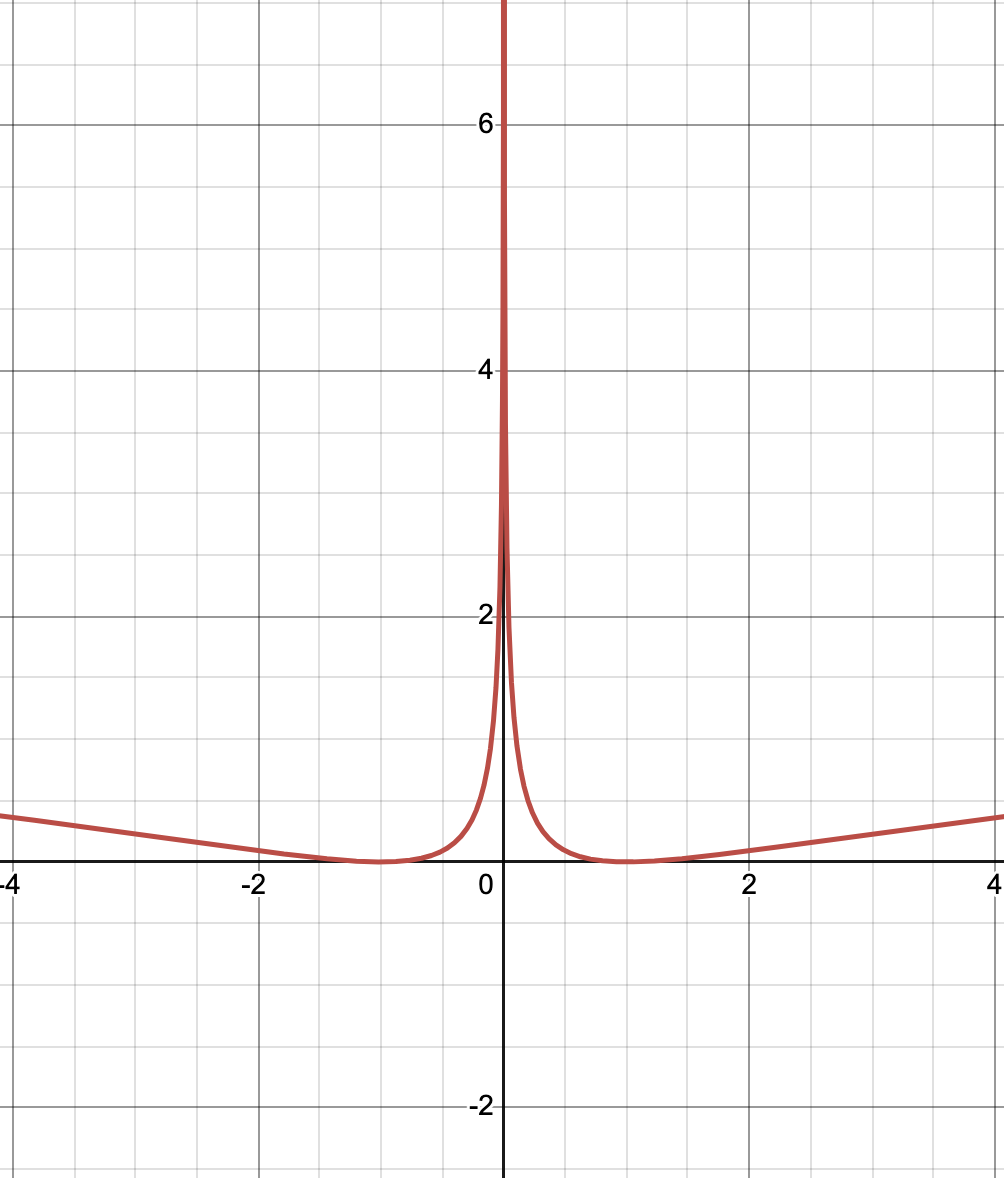
\includegraphics[scale=0.3]{Graph}
\end{center}
\end{proof}
\section*{7.}
\begin{proof}
Use the same function as the previous question. Once again, we have a discontinuity near $0$, and again, we can have a Cauchy sequence. The same as before, the only scenario of concern is when the scenario when $\frac{1}{m} < |x| \leq \frac{1}{n}$ and as $m \to \infty$ the integral will go to $0$, so we have that the sequence is Cauchy. 
\end{proof}

\section*{8.}
\begin{proof}
  We will prove the claim by induction on $k$. We have already completed the base case where $k = 1$ as 
  \[
  \zeta(2) = \frac{\pi^2}{6}  = rational*\pi^2.  
  \]
  For the inductive hypothesis, assume the claim holds for $2k$, and we will prove the $2(k + 1) = 2k + 2$ case. We begin by calculating the first Fourier coefficient 
  \[
  a_0 = \frac{1}{\pi}\int_{-\pi}^{\pi} x^{2k + 2}\cos(nx) \mathrm{d}x  
  \]
  to solve the integration by parts pick $u = x^{2k + 2}$, $du = (2k + 2)x^{2k + 1}$, $dv = \cos(nx)$ and $v = \frac{1}{n}\sin(nx)$, and we get
  \begin{align*}
    a_n &= \left[x^{2k + 2}\cdot \frac{1}{n}\sin(nx) \right]_{-\pi}^{\pi} - \frac{1 }{\pi} \int_{-\pi}^{\pi} (2k + 2)x^{2k + 1}\frac{\sin(nx)}{n}\mathrm{d}x \\
    &= -\frac{2k + 2}{n \pi}\int_{-\pi}^{\pi}x^{2k + 1} \sin(nx) \mathrm{d}x.
  \end{align*}
  Once again we can apply integration by parts by picking $u = x^{2k + 1}$, $du = (2k + 1)x^{2k}$, $dv = \sin(nx)$, and $v = -\frac{1}{n}\cos(nx)$, we get
  \begin{align*}
    a_n &= -\frac{2k + 2}{n \pi }\left(\left[-\frac{1}{n}x^{2k + 1}\cos(nx) \right]_{-\pi}^{\pi} - \int_{-\pi}^{\pi} -\frac{1}{n}\cos(nx) (2k + 1)x^{2k} \right) \\
    &= -\frac{2k + 2}{n \pi}\left(-\frac{1}{n}\pi^{2k + 1}(-1)^n - \frac{1}{n}\pi^{2k +1}(-1)^n \right) - \frac{(2k + 2)(2k + 1)}{n^2 \pi}\int_{-\pi}^{\pi}x^{2k}\cos(nx) \mathrm{d}x.
  \end{align*}
  By our inductive hypothesis we have that $\zeta(2k)$ is a rational times $\pi^{2k}$. We can express the coefficients of the Fourier series of $x^{2k + 2}$ as rational numbers time primes subtracting the coefficients of $x^{2k}$ and the first coefficient of $x^{2k + 2}$ has the term $\pi^{2k + 2}$. Thus, we have that $\zeta(2k + 2)$ will be a rational times $\pi^{2k + 2}$. 
\end{proof}
\section*{9.}
\begin{proof}
  We have already solved for $\zeta(6)$ in problem 3:
  \[
  \zeta(6) = \frac{\pi^6}{945}.  
  \]
\end{proof}
\end{document}